The current method of controlling the player (the car) in Cars, is based on sound input.
When the game is running, voice input is continually recorded and analysed, in order to detect the pitch of the sound input, so that the direction in which to move the car can be decided.
The current method of analysing this is by using Fast Fourier's Transformation (FFT) and subsequently choosing the loudest frequency.

In this section we will briefly explain what sound is, in order to understand how to obtain certain characteristics of sound.
Based on this knowledge we will argue why it is difficult to obtain frequency from a sound input, especially sound input with human voice.
The technicalities in the section are based on \cite{music-and-computers}.

\subsection{Characteristics of sound}
Sound is a physical phenomenon which acts like a wave and therefore have the same characteristics as a wave.
So basically sound is a movement of air and the way we perceive sound is an interpretation of these movements.

Simply speaking, the volume (or loudness) of a sound, is the amplitude of the sound wave.
The pitch of a sound, how high/low we perceive it, is the frequency of the sound wave.
These two characteristics are independent, meaning that two sound waves with same frequency, but different amplitudes, will sound like the same pitch, but one being louder than the other.
An example can be seen in \cref{fig:samepitchdiffamp}.

\begin{figure}[h]
\centering
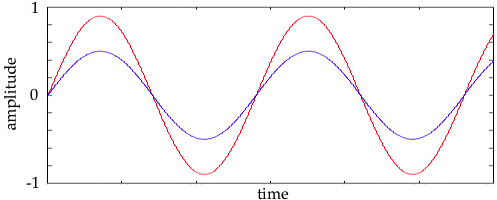
\includegraphics[width=.80\textwidth]{sprint1/samepitchdiffamp}
\caption{Two sound waves (represented as sine functions) with same frequency, but different amplitude.}
\label{fig:samepitchdiffamp}
\end{figure}

There is also a third characteristic, which is more abstract and not directly a physical attribute, namely, timbre.
Timbre is a composition of different sound waves (spectra), which makes up a specific sound (again, this is perceptual) and envelope (transients), which describe the different stages of a sound.

\subsection{Obtaining frequency}
Obtaining frequency is fairly simple, as it can read from a sound input interpreted as a wave (sine function).
However, some sounds are simpler than others in their composition of waves.
These simpler sounds could be considered ''cleaner'' than others, meaning they consist of only a single or very few waves, where it is easy to identify a primary amplitude and frequency.

Human speech, among other sounds, consists of multiple sound waves, each with varying amplitude and frequency.
In this case, it may be difficult to point out a single wave as the most important, and choose its frequency as the main frequency.
A comparison between frequency spectra can be seen in \cref{fig:frequency_spectra}.

\begin{figure}[h]
\centering
\begin{subfigure}[t]{.45\textwidth}
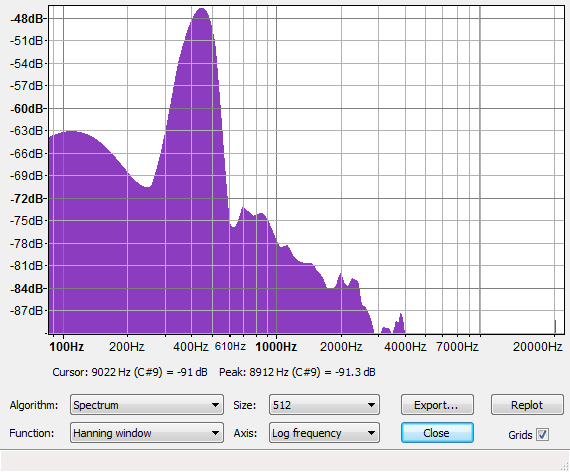
\includegraphics[width=\textwidth]{sprint1/spectrum_tonegenerator}
\caption{Frequency spectrum for a 440 Hz generated tone}
\end{subfigure}
\begin{subfigure}[t]{.45\textwidth}
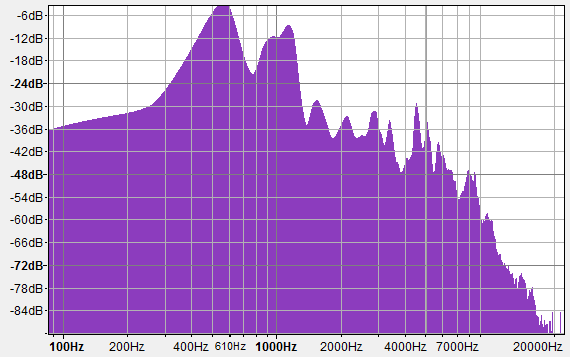
\includegraphics[width=\textwidth]{sprint1/spectrum_highpitchvoice}
\caption{Frequency spectrum for human voice input (in an attempt to reach high pitch)}
\end{subfigure}
\caption{Frequency analysis in Audacity}
\label{fig:frequency_spectra}
\end{figure}

\subsection{Using FFT}

